\documentclass{article}
\usepackage{amsmath, amsthm, amssymb, booktabs, hyperref, graphicx, float, esint, xcolor, subcaption, xspace}
\setlength{\abovedisplayskip}{0pt}
\setlength{\belowdisplayskip}{0pt}
\setlength{\abovedisplayshortskip}{0pt}
\setlength{\belowdisplayshortskip}{0pt}

\newcommand{\vr}{\vec{r}}
\newcommand{\vOmega}{\vec{\Omega}}
\newcommand{\vO}{\vec{\Omega}}
\newcommand{\bra}{\left\langle}
\newcommand{\ket}{\right\rangle}
\newcommand{\sbra}{\left[}
\newcommand{\sket}{\right]}
\renewcommand{\div}{\vec{\nabla} \cdot}
\newcommand{\grad}{\vec{\nabla}}
\newcommand{\vbeta}{\vec{\beta} }
\newcommand{\pdx}{\frac{\partial}{\partial x}}
\newcommand{\pdy}{\frac{\partial}{\partial y}}
\newcommand{\pdz}{\frac{\partial}{\partial z}}
\newcommand{\intrrr}{\int d^3 r \,}
\newcommand{\intrr}{\int d^2 r \,}
\newcommand{\dEdphi}{\partial_\phi E \,}
\newcommand{\dEdp}{\partial_p E \,}
\newcommand{\dBdphi}{\partial_\phi B \,}
\newcommand{\dBdp}{\partial_p B \,}
\newcommand{\adj}{\phi^\dag}
\newcommand{\surf}{\int_{\partial V}}
\newcommand{\bound}{\partial V}
\newcommand{\vn}{\vec{n}}
\newcommand{\Edd}{\mathbb{E}}
\newcommand{\BEdd}{\mathbf{B}}
\newcommand{\sigt}{\sigma_t}
\newcommand{\sigs}{\sigma_s}
\newcommand{\siga}{\sigma_a}
\newcommand{\isigt}{c}
% why \newcommand{\angSource}{q_\Omega}
\newcommand{\angSource}{q}
\newcommand{\scalSource}{q}
\newcommand{\angResp}{q^\dag}
\newcommand{\scalResp}{q^\dag}
\newcommand{\qoi}{{\it QoI}\xspace}


\newcommand{\comment}[2]{\marginpar{\textcolor{#2}{$\star$}}\textcolor{#2}{#1}\newline}
\newcommand{\iwh}[1]{\comment{#1}{red}}
\newcommand{\jcr}[1]{\comment{#1}{blue}}

\begin{document}
\begin{center}
{\large Thesis Proposal~:\\
{\it Adjoint-based sensitivity for radiation transport using an Eddington tensor formulation}}\\
\vspace{2mm}
Ian Halvic, Texas A\&M University, NUEN
\end{center}

\tableofcontents
\newpage

%%%%%%%%%%%%%%%%%%%%%%%%%%%%%%%%%%%%%%%%%%%%%%%%%%%%%%%%%%%%%%%%%%%%%%%%%%%%%%%%%%%%%%%%%%%%%%%%%%%%
\section{Introduction}
%%%%%%%%%%%%%%%%%%%%%%%%%%%%%%%%%%%%%%%%%%%%%%%%%%%%%%%%%%%%%%%%%%%%%%%%%%%%%%%%%%%%%%%%%%%%%%%%%%%%

Computational simulations have become important tools for engineers and scientists across a wide array of disciplines. These simulations allow for researchers to examine significantly complex and long life systems in a way that is frequently more economical in both time and money than construction of the real world system, if even feasible. An important step in creating one of these methods is confirmation that the results can be trusted to reasonably approximate the real life scenario. This can be accomplished using three process outlined by the National Research Council \cite{NRCVVUQ}


\begin{itemize}
\item Verification - How accurately does the computation solve the underlying equations of the model for the quantities of interest?
\item Validation - How accurately does the model represent reality for the quantities of interest?
\item Uncertainty Quantification (UQ) -  How do the various sources of error and uncertainty feed into uncertainty in the model-based prediction of the quantity of interest?
\end{itemize}


Adjoint methods are particularly useful for UQ. In general, adjoint methods provide a mechanism for computing quantities of interest (\qoi) and sensitivity coefficients and, more generally, for propagating uncertainty and error in the system variables to the error in the desired quantity of interest. They accomplish this in a particularly economical way, requiring only two full system solves (one forward and one adjoint solve) in order to determine sensitivity coefficients for any combination of sources of uncertainty, as opposed to performing an multiple forward system solve to determine
the sensitivity due to each individual uncertain parameter.

Using operator notation to denote the forward and adjoint (linear) problems, $Au=q$ and $A^\dag u^\dag = q^\dag$, respectively, and the bracket notation for inner products over the phase space, it is easy to note that a \qoi can 
obtained using either the forward solution $u$ folded with the response function of interest (which is also the adjoint source, $q^\dag$)
\[
\qoi = \bra u, q^\dag \ket = \bra u^\dag, q \ket \,.
\]
A first-order sensitivity coefficient due to parameter $p$ can be obtained using two forward solves
\[
\delta_p \qoi = \frac{\qoi^\prime - \qoi}{\delta p} = \frac{ \bra (u^\prime - u), q^\dag \ket}{p^\prime - p}  \,,
\]
where the superscript $^\prime$ denotes a perturbed value. Equivalently, one can employ the unperturbed adjoint solution to obtain
an estimation of the sensitivity coefficient
\[
\delta_p \qoi = \bra u^\dag, \delta_p q - \delta_p A u \ket \,.
\]
The subsequent sections will provide additional details and will apply these formulations to neutron transport problems. However, it is already evident that if the forward source $q$ is uncertain and only a few \qoi are requested, it is preferable to employ the adjoint formulation to compute the quantity of interest. Furthermore, the sensitivity of the
\qoi to many uncertain parameters is more advantageously computed using the adjoint.


Adjoint methods are of particular interest for UQ. In general, adjoint methods provide a mechanism for propagating uncertainty and error in the system variables to the error in the desired quantity of interest. Djoint methods accomplish this in a particularly economical way, sometimes requiring only two differential system solves which can then be used for any combination of sources of error, as opposed to performing an independent solve for each individual error scenario. These adjoint methods have been applied across various complex and time dependent systems. An example of adjoint methods applied to hydrodynamic systems with shocks can be found in Wildey et al. \cite{Wildey}. A more relevant adjoint example to neutron transport occurs in Stripling et al. in the form of reactor burn-up equations \cite{Stripling}.


Application of the adjoint method to time-dependent transport can pose a major technical limitation. In general, the adjoint method would require storing six-dimensional data (the forward angular flux) at each time step. When dealing with high resolution in these six dimensions and many time steps, this can potentially require an unreasonable amount of memory for data storage, rendering the method functionally unusable. For the previously mentioned depletion problem, this limitation was resolved by storing the converged scattering moments only at defined checkpoints then using interpolation to reconstruct the forward flux for use in the adjoint \cite{Stripling};
using converged scattering souce term, a single transport sweep is needed to recover the converged
angular flux. However this method does not extend to time-dependent transport in general because
the primary time-dependent variable, the angular flux, needs to be stored. 

A potential solution to the memory requirement for the time-dependent transport adjoint formulation is the use of a quasi-diffusion method to reduce the overall dimensionality of the transport problem, from 6D+time (space, direction, energy, time for transport) to 4D+time (space, energy, time for quasi-diffusion). The method examined in this work is termed  as a ``Variable Eddington Tensor'' formulation, and uses the unperturbed forward angular flux to compute the Eddington tensor needed in the quasi-diffusion approach.


%%%%%%%----------------------------------------------------------------------------------------------
\subsection{Steady-state one-group neutron transport equation}
%%%%%%%----------------------------------------------------------------------------------------------

This work will focus on a relatively simple transport equation form, the one-group steady-state transport equation. Examination of the quasi-diffusion's effectiveness in this setting will provide sufficient insight to advantages and shortcomings of the technique when applied to multigroup, time-dependent transport equation. The one-group steady-state transport equation with isotropic scattering for a volume $V$ bounded by its surface $\partial V$ is given below.

This paper will focus on a relatively simple transport equation form, the one-group steady state transport equation. Examination of the quasi-diffusion's effectiveness in this simple case may provide insight to advantages and shortcomings when applied to a full time-dependent transport equation. The one-group steady state transport equation for a volume $V$ bounded by the surface $\partial V$ is given below.

\begin{equation}
\label{SS1GTE}
\vO \cdot \grad \psi(\vr,\vO) + \sigt(\vr) \psi(\vr,\vO) = \frac{1}{4 \pi} \sigs(\vr) \phi(\vr) + q(\vr,\vO), \quad \forall \vr \in V
\end{equation}
\begin{equation}
\psi(\vr,\vO) = \psi^{\text{inc}}(\vr,\vO) \quad \vr \in \partial V^{-} = \{ \vr \in \partial V, \text{ s.t. }, \vO \cdot \vec{n}(\vr) < 0\}
\end{equation}
The possibly uncertain parameters in this system are: the total and scattering cross sections $\sigt$ and $\sigs$, the volumetric source term $q$, and the incident angular flux on the system given by $\psi^{\text{inc}}$. The unknowns (dependent variables) are the angular flux $\psi(\vr,\vO)$ and the scalar flux $\phi(\vr)$ given by
\[
\phi(\vr) = \int_{4\pi}d\Omega\,\psi(\vr,\vO) \,.
\]
%%%%%%%----------------------------------------------------------------------------------------------
%\subsection{Quantity of interest and their sensitivities}
%%%%%%%----------------------------------------------------------------------------------------------

%----------------------------------------------------------------------------------------------
\subsubsection{Quantity of interest, response function, and inner products}
%----------------------------------------------------------------------------------------------
Frequently, the solution to the transport equation is not the sought after value, but rather some Quantity of Interest (\qoi), a functional that depends on the transport solution. Given $\psi(\vr,\vO)$ the solution of the one-group steady-state transport (Eq.~\eqref{SS1GTE}), a \qoi
defined as
\begin{equation}
\qoi =  \int_V dV \int_{4 \pi} d \vO \,  R(\vr, \vO) \psi(\vr, \vO)
\end{equation}
where $R(\vr, \vO)$ is termed the ``response function'' which is used to characterize the meaning of the desired \qoi. The response function can take on physically defined forms, such as the cross section of a detector; or it may take a form of a mathematical construct, such as $R(\vr, \vO)=1/v$ to return the total neutrons of speed $v$ present in the system. To avoid confusion with the spatial location vector $\vr$, the response function will frequently be expressed as $q^\dag$, the adjoint source, as we have already noted that there is a relationship between the solution, the adjoint solution, and their respective source terms.

For the sake of brevity in this paper, particularly for expressing the \qoi, two volumetric inner products are defined both using $\bra \bullet , \bullet \ket$ notation. These two inner-products are for use with angular and scalar flux respectively. 
\begin{subequations}
\begin{equation}
\bra \psi , \angResp \ket_{V \times \mathcal{S}_2}  = \int_V dV \int_{4 \pi} d \Omega \,  \psi(\vr, \vO)\angResp(\vr, \vO)
\end{equation}
where $\mathcal{S}_2$ denotes the unit sphere.
\begin{equation}
\bra \phi(\vr) ,\angResp \ket_V  = \int_V dV \,  \phi(\vr)\angResp(\vr)
\end{equation}
\end{subequations}
For later use, two additional inner products are also defined as surface integrals over the region boundary $\partial V$. The latter splinting incoming and outgoing surface integrals.
\begin{subequations}
\begin{equation}
\sbra \psi , g \sket_{\bound \times \mathcal{S}_2}  = \int_{\bound} dS \int_{4 \pi} d \Omega \, \vO \cdot \vn(\vr) \, \psi(\vr, \vO)g(\vr, \vO)
\end{equation}
\begin{equation}
\sbra \phi , g \sket_{\pm}   = \int_{\bound} dS \int_{\vO \cdot \vn \gtrless 0} d\Omega \,  \vO \cdot \vn(\vr) \, \phi(\vr, \vO)g(\vr, \vO)
\end{equation}
\end{subequations}
\jcr{I do not know where the first surface inner product is used. I have always used the second one. Please show me an equation where the first one is needed!}
\iwh{I sort of use the first one as a "general" form when doing integration by parts. The second one is used moreso when the actual boundary conditions are applied (since the first can be expressed as a sum of the + and - versions of the second). Its the difference/step between Eq.~\eqref{snAdjQoI} and Eq.~\eqref{snAdjQoIBCsplit}}
\jcr{I do not understand why you use phi and not psi in the second one}

The inner product subscripts will frequently be dropped when it is unambiguous which one being used, typically indicated by the presence of an angular-dependent variable, e.g., $\psi$ or an angular-independent variable, e.g., $\phi$. Therefore, with this notation, the quantity of interest can be compactly expressed as shown below.
\begin{equation}
\label{QoIDef}
\qoi = \bra \psi(\vr,\vO), \angResp(\vr,\vO) \ket  = \bra \phi(\vr) , \scalResp(\vr) \ket
\end{equation}
The boundary terms arise from the integration by parts of the streaming terms.
\jcr{In the thesis, the above must be demonstrated, including what the boundary terms look like}
\iwh{This is the forward QoI solution, using the response function. I don't think that we generally have boundary terms this way (though I guess you could create a surface response).}

%----------------------------------------------------------------------------------------------
\subsubsection{Sensitivity Coefficients}
%----------------------------------------------------------------------------------------------
A hurdle in utilizing the transport equation numerically to make real world predictions is that none of the system's parameters ($\sigt$, $\sigs$, $q$, and $\psi^{inc}$) are not known exactly. This error in the system parameters is expected to translate to error in the \qoi value. Ideally, a reasonable error range would be determined for each system parameter and the system simulation would run over a finely discretized parameter space, using the resulting \qoi values to generate an error range for the \qoi. However, this straightforward method tends to be resource-intensive, requiring a complete forward solve of the transport equation for each input error scenario. Adjoint methods offer a way to drastically reduce the number of solves, while generally remaining fairly accurate for small perturbations around base or nominal values of the parameters.


%%%%%%%----------------------------------------------------------------------------------------------
\subsection{Adjoint Sensitivity}
%%%%%%%----------------------------------------------------------------------------------------------
\jcr{If you prefer to use $\mathbf{A}$ as opposed to $A$, do this from the very beginning as well}

Adjoint operators can provide a useful tool for sensitivity calculations. Using inner product notation $\bra \bullet , \bullet \ket$, consider the system of interest $\mathbf{A} \psi = q$. Call this this the forward system, with forward operator $\mathbf{A}$. Consider a test function $\psi^\dag$, the adjoint operator $\mathbf{A^\dag}$ is defined such that $\bra \mathbf{A} \psi, \psi^\dag \ket = \bra \psi, \mathbf{A^\dag} \psi^\dag \ket $. For differential operators, derivation of $\mathbf{A^\dag}$ generally relies on application of the divergence theorem (integration by parts), typically resulting in boundary terms ($BC$). Using the response function of the desired \qoi, the adjoint system can be constructed as $\mathbf{A^\dag} \psi^\dag = q^\dag$, leading to an alternate expression of the \qoi using the adjoint solution $\psi^\dag $.
\begin{equation}
\label{genAdjQoI}
\qoi = \bra \psi, R \ket = \bra q , \psi^\dag \ket + BC
\end{equation} 
From the above, it follows that a first order approximation to the change in the quantity of interest based on perturbations to the initial system, including perturbation to the forward operator $\delta \mathbf{A}$ and forward source $\delta q$, can be expressed in the form shown in Eq.~\eqref{genAdjSens} \cite{Marchuk}.
\begin{equation}
\label{genAdjSens}
\delta \qoi \approx \bra \delta q - \delta \mathbf{A} \psi , \psi^\dag \ket 
\end{equation}
The advantage of the above expression for $\delta \qoi$ is that two solves, one for the forward and another for the adjoint, can be used to approximate the sensitivity for a variety $\delta \mathbf{A}$ and $\delta q$.
\jcr{in the thesis, you need to go through the algebra for the transport and the VET equations. not here, this is only the proposal}
\iwh{Will do}
 
%%%%%%%%%%%%%%%%%%%%%%%%%%%%%%%%%%%%%%%%%%%%%%%%%%%%%%%%%%%%%%%%%%%%%%%%%%%%%%%%%%%%%%%%%%%%%%%%%%%%
\section{Discrete Ordinates (Sn) Transport}
%%%%%%%%%%%%%%%%%%%%%%%%%%%%%%%%%%%%%%%%%%%%%%%%%%%%%%%%%%%%%%%%%%%%%%%%%%%%%%%%%%%%%%%%%%%%%%%%%%%%
A discrete ordinates (Sn) method can be used to solve the one group steady state transport equation (Eq.~\eqref{SS1GTE}). The focus of this method is to discretize the angular variable into discrete directions. Using an angular quadrature with $D$ directions $\vO_d$, the transport equation is solved along each direction:
\begin{equation}
\label{1gTE}
\vO_d \cdot \grad \psi_d + \sigt \psi_d = \frac{\sigs}{4 \pi} \phi + q_d \quad \vr \in V , \forall d\in [1,D]
\end{equation}
%
The scalar flux can be computed from the angular flux as follows
\[
\phi(\vr) \approx \sum_{d=1}^D w_d \psi_d(\vr) \,,
\] 
where $\psi_d(\vr) = \psi(\vr, \vO_d)$ and $w_d$ is the angular quadrature weight. This leads to a coupled system of $D$ equations of the form shown in Eq.~\eqref{1gTE}, where the system is coupled through the scattering source term.



%%%%%%%----------------------------------------------------------------------------------------------
\subsection{Adjoint Formulation for Sn Transport}
%%%%%%%----------------------------------------------------------------------------------------------
In a fairly straightforward application of the adjoint method previously shown, the adjoint equation which corresponds to the Sn transport formulation with adjoint source (response function)
$\angResp$ is
\begin{equation}
\label{snAdj}
- \vO_d \cdot \grad \psi^\dag_d + \sigt \psi^\dag_d = \frac{\sigs}{4 \pi} \phi^\dag + \angResp_d
\end{equation}
%
\begin{equation}
\psi^\dag(\vr) = \psi^{\dag \text{out}}(\vr)=0 \quad \vr \in \partial V^{+} = \{  \vr \in \bound , \quad \vO \cdot \vec{n} > 0 \}
\end{equation}
where the definition of the adjoint scalar flux $\phi^\dag$ is analogous to that of 
the forward scalar flux definition. It is worth noting that the Sn adjoint equation is in the form of the standard transport equation, only with the direction of travel reversed ($\vO \to -\vO)$. This often allows for forward Sn transport solvers to be easily adapted to solving the Sn adjoint system. Once the adjoint solution is obtained, the corresponding QoI can be calculated with a simple inner product with the forward source term, as follows from equation Eq.~\eqref{genAdjQoI}. %
\begin{equation}
\label{snAdjQoI}
QoI = \bra \psi^\dag , \angSource \ket - \sbra \psi^\dag,  \psi \sket
\end{equation}
%
The surface interval in \ref{snAdjQoI} can be split into incoming and outgoing flux integrals, which are handled by the forward and adjoint boundary conditions respectively. 
%
\begin{equation}
\label{snAdjQoIBCsplit}
\qoi = \bra \psi^\dag , q \ket - \sbra \psi^{\dag \text{out}},  \psi \sket_+ - \sbra \psi^\dag,  \psi^{\text{inc}} \sket_- \,.
\end{equation}

%%%%%%%----------------------------------------------------------------------------------------------
\subsection{Sn Transport Adjoint Sensitivity}
%%%%%%%----------------------------------------------------------------------------------------------

Now consider perturbations to our system. Specifically perturbations of $\delta \sigt$, $\delta \sigs$, and $\delta q$ to the total cross section, scattering cross section and angular source term respectively. In addition, the incident angular flux is also perturbed by $\delta \psi^{inc}$. These perturbations result in a perturbed solution to the Sn-transport equation $\psi_p$. 
\begin{equation}
\label{snFwdPert}
\vO \cdot \grad \psi_p + \sigma_{t,p} \psi_p = \frac{\sigma_{s,p}}{4 \pi} \phi_p + q_p,  \quad \forall \vr \in V
\end{equation}
\begin{equation}
\psi_p(\vr) = \psi_p^{\text{inc}}(\vr), \quad \forall \vr \in \partial V^{-}
\end{equation}
Any quantity with a subscript $p$ is to be understood as the perturbed value, that is, as 
the sum of the unperturbed value and the perturbation amount: $a_p = a + \delta a$.

This perturbation may result in a change to the \qoi, now given by $\qoi_p=\bra \psi_p , \angResp \ket$. Using the unperturbed adjoint equation given in Eq.~\eqref{snAdj},
the perturbed \qoi can be expressed as:
\begin{equation}
\label{snSensPart}
\begin{split}
QoI_p &=\bra \psi_p , \angResp \ket \\
&=\bra \psi_p , - \vO \cdot \grad \psi^\dag + \sigt \psi^\dag - \frac{\sigs}{4 \pi} \phi^\dag  \ket \\
%&= \bra  \vO \cdot \grad \psi_p + \sigt \psi_p - \frac{\sigs}{4 \pi} \phi_p , \psi^\dag  \ket - \sbra \psi_p, \psi^\dag \sket\\
\end{split}
\end{equation}
Next, we perform an integration by parts and obtain:
\begin{equation}
\label{snSensPart2}
QoI_p = \bra  \vO \cdot \grad \psi_p + \sigt \psi_p - \frac{\sigs}{4 \pi} \phi_p , \psi^\dag  \ket - \sbra \psi_p, \psi^\dag \sket
\end{equation}
Note that the cross sections are unperturbed in Eq.~\eqref{snSensPart2}.
Using a $\delta$ notation for the perturbed system variables ($\sigma_{s,p} = \sigs + \delta \sigs$ for example), we
can introduced the perturbed quantities:
\begin{equation}
\label{snSensPart3}
\begin{split}
QoI_p &= \bra  \vO \cdot \grad \psi_p + \sigma_{t,p}\psi_p - \delta\sigt\psi_p - \frac{\sigma_{s,p}}{4 \pi} \phi_p
+\frac{\delta \sigs}{4 \pi} \phi_p
 , \psi^\dag  \ket - \sbra \psi_p, \psi^\dag \sket \\
 &= \bra  q_p - \delta\sigt\psi_p + \frac{\delta \sigs}{4 \pi} \phi_p
 , \psi^\dag  \ket - \sbra \psi_p, \psi^\dag \sket
\end{split}
\end{equation}
Next, note that some terms have double perturbations, such as $\delta \sigt \delta \psi$ once it is observed
that $\psi_p=\psi+\delta\psi$. 
In a first order approximation, these doubly perturbed terms are ignore, yielding:
\begin{equation}
\label{snAdjQoI}
QoI_p \approx \bra  q + \delta q - \delta\sigt\psi + \frac{\delta \sigs}{4 \pi} \phi
 , \psi^\dag  \ket - \sbra \psi_p, \psi^\dag \sket\end{equation}

Subtraction of the unperturbed \qoi expression in Eq.~\eqref{snAdjQoI} supplies a final equation for computing the change in \qoi using only the system perturbations and the unperturbed forward solution $\psi$ and the adjoint unperturbed
solution $\psi^\dag$, removing the need to solve the perturbed forward equation. 
Furthermore the boundary terms can be split into incoming and outgoing contributions.
Using a zero-outcoming  boundary condition for the adjoint flux
(thus $\sbra \delta \psi, \psi^{\dag,\text{out}} \sket_+=0$), one obtains the final 
form of the perturbation in the \qoi.
\begin{equation}
\begin{split}
\delta QoI &= \bra \delta \scalSource - \delta \sigt \psi + \frac{\delta\sigs}{4 \pi} \phi  , \psi^\dag  \ket - \sbra \delta \psi, \psi^\dag \sket \\
&= \bra \delta \scalSource - \delta \sigt \psi + \frac{\delta\sigs}{4 \pi} \phi , \psi^\dag  \ket - \sbra \delta \psi^{\text{inc}}, \psi^\dag \sket_- \,.
\end{split}
\end{equation}

%%%%%%%%%%%%%%%%%%%%%%%%%%%%%%%%%%%%%%%%%%%%%%%%%%%%%%%%%%%%%%%%%%%%%%%%%%%%%%%%%%%%%%%%%%%%%%%%%%%%
\section{VET formulation}
%%%%%%%%%%%%%%%%%%%%%%%%%%%%%%%%%%%%%%%%%%%%%%%%%%%%%%%%%%%%%%%%%%%%%%%%%%%%%%%%%%%%%%%%%%%%%%%%%%%%

%%%%%%%----------------------------------------------------------------------------------------------
\subsection{Motivation} 
%%%%%%%----------------------------------------------------------------------------------------------

While the Sn adjoint sensitivity formulation given by Eq.~\eqref{snSens} provides a first-order accurate method to determine the sensitivity to multiple perturbation scenarios using only a single forward and adjoint transport solve, it can quickly run into technical limitations. Specifically for even a one-group time independent system, all solutions to the forward and adjoint system in space and angle must be stored for retrieval later. For a spatially 3-dimensional system, this translates to storing discretized data across 5-dimensions.


%%%%%%%----------------------------------------------------------------------------------------------
\subsection{VET Formulation}
%%%%%%%----------------------------------------------------------------------------------------------

The Variable Eddington Tensor (VET) formulation shows promise of reducing the memory requirements when using the adjoint method for sensitivity. To begin the formulation, the steady state transport equation is expanded to the scalar and first angular moment by application of the $\int d \Omega$ and $\int d \Omega \, \vO$ operators to Eq.~\eqref{1gTE}, respectively. Using the notation

\begin{equation}
\phi(\vr)=\int d\Omega \, \psi( \vr,\vO )
,\quad
\vec{J}(\vr)= \int d\Omega \, \vO \psi( \vr,\vO )
\end{equation}
the zero-th and first angular moment transport equations are
\begin{equation}
\label{0am}
\div \vec{J} + \sigt \phi = \sigs \phi + \scalSource
\end{equation}
\begin{equation}
\label{1am}
\div \left(  \int d\Omega \vO \vO \psi \right) + \sigt \vec{J} =0 
\end{equation}
The Eddington Tensor $\Edd$ is then introduced as a simplifying approximation relating the second angular moment term in equation \ref{1am} to the scalar flux. 
\begin{equation}
\label{EddDef}
\Edd(\vr)=\frac{\int d\Omega \vO \vO \psi(\vr,\vO)}{\phi(\vr)}
\end{equation}
The inclusion of the Eddington tensor allows Eq.~\eqref{1am} to be expressed as 
\[
\vec{J} = - \frac{1}{\sigt} \div \Edd \phi.
\]
If $\psi(\vr,\vO)$ is a linear function in angle, then $\Edd(\vr)=\tfrac{1}{3}\mathbb{I}$ and one recovers Fick's law for the neutron diffusion current, $\vec{J} = - \frac{1}{3\sigt} \grad \phi$ (note the change from $\div$ to $\grad$). Using this as a definition of $\vec{J}$ allows us to convert Eq.~\eqref{0am} to the form shown in \ref{VEFForm}, which only has the scalar flux as an unknown. The substitution $\siga = \sigt-\sigs$ was used.
\begin{equation}
\label{VEFForm}
- \div \left( \frac{1}{\sigt}\div \Edd \phi \right) + \siga \phi = \scalSource
\end{equation}
The known incident flux can be used to generate a suitable boundary condition using a "Boundary Eddington Factor" $\BEdd$, constructed elementwise as shown below. \cite{Miften}.
\begin{equation}
\frac{1}{\sigma_{t} } \vec{\nabla} \cdot \left(\Edd \phi \right)  = - 2J^- - \BEdd \phi \quad \vr \in \bound
\end{equation}
\begin{equation}
B_i= \frac{\int_{4 \pi} d\Omega \, \left| \Omega_i n_i \right | \psi}{\int_{4\pi} d\Omega \, \psi} \quad \vr \in \bound , \, \, i=x,y,z 
\end{equation}
\jcr{explain subscript i}

%%%%%%%----------------------------------------------------------------------------------------------
\subsection{Adjoint VET formulation}
%%%%%%%----------------------------------------------------------------------------------------------

The VET formulation necessitates a reformulation of our adjoint. As shown in Eq.~\eqref{adjForm}, the double divergence term present in the forward equation contributes to a double gradient term in the adjoint equation.

\begin{equation}
\label{adjForm}
- \Edd : \left( \grad \left( \frac{1}{\sigt}\grad \phi^\dag \right) \right) + \siga \phi^\dag = \scalResp
\end{equation}
\jcr{in thesis, you must demonstrate this}
For reasons that will become apparent during sensitivity calculations, the boundary condition chosen for the adjoint equation is given in \ref{adjVETBC}. Unlike for Sn formulation, the VET adjoint equation does not take the form of a VET transport equation.

For reasons that will become apparent during sensitivity calculations, the boundary condition chosen for the adjoint equation is given in Eq.~\eqref{adjVETBC}. Unlike for Sn formulation, the VET adjoint equation does not take the form of a VET transport equation.

\begin{equation}
\label{adjVETBC}
\Edd \cdot \frac{1}{\sigma_{t} } \vec{\nabla} \phi^\dag  = - 2J^{\dag +} - B \phi^\dag \quad \vr \in \Gamma
\end{equation}
To obtain the QoI using this formulation, begin with the typical QoI definition, relocate operators to the forward to substitute the forward source, and apply boundary conditions.
\begin{equation}
\label{VETQoIAdjUnpDeriv}
\begin{split}
QoI=&\bra \phi , \scalResp \ket \\
=&\bra \phi , - \Edd : \left( \grad \isigt \grad \phi^\dag \right) + \siga \phi^\dag \ket \\
=& \bra - \div \isigt \div \left( \Edd \phi \right) + \siga \phi, \phi^\dag \ket 
- \sbra \phi, \Edd \cdot \isigt \grad \phi^\dag \sket  
+ \sbra \phi^\dag, \isigt \grad \Edd \phi \sket \\
=&\bra \scalSource , \phi^\dag \ket 
- \sbra \phi , - 2J^{\dag +} - B \phi^\dag \sket + \sbra \phi^\dag, - 2J^- - B \phi  \sket
\end{split}
\end{equation}
The boundary Eddington terms negate and yield a relatively compact form for the QoI
\begin{equation}
\label{VETQoIAdj}
QoI=\bra \scalSource , \phi^\dag \ket 
+ \sbra 2\phi, J^{\dag +} \sket  - \sbra 2\phi^\dag, J^- \sket
\end{equation}

%%%%%%%----------------------------------------------------------------------------------------------
\subsection{VET adjoint sensitivity}
%%%%%%%----------------------------------------------------------------------------------------------

As was done in the Sn transport formulation, once again consider perturbations to the system parameters. However, in contrast to the Sn case, the assumption is also made that the Eddington factor remains unperturbed under these system perturbations. For brevity, the substitution of $\isigt = \sigt^{-1}$ was also made.
\begin{equation}
\label{VEFPert}
- \div \left((\isigt + \delta \isigt)\div \Edd \phi_p \right) + (\siga + \delta \siga)\phi_p = \scalSource + \delta \scalSource
\end{equation}
\begin{equation}
(\isigt + \delta \isigt) \vec{\nabla} \cdot \left(\Edd \phi_p \right)  = - 2J_p^- - B \phi_p \quad \vr \in \bound
\end{equation}
The usual adjoint process is performed, starting with the QoI definition using the perturbed solution and response. 
\begin{equation}
\label{VETSensDeriv}
\begin{split}
\qoi=&\bra \phi_p , \scalResp \ket \\
=&\bra \phi_p , - \Edd : \left( \grad \isigt \grad \phi^\dag \right) + \siga \phi^\dag \ket \\
=& \bra - \div \isigt \div \left( \Edd \phi_p \right) + \siga \phi_p, \phi^\dag \ket 
- \int_\Gamma d^2 r \, \phi_p \left( \Edd \cdot \isigt \grad \phi^\dag \right) \cdot \vec{n}  \\ 
&+ \int_\Gamma d^2 r \, \phi^\dag \left(  \isigt \grad \Edd \phi_p \right) \cdot \vec{n} \\
\end{split}
\end{equation}
A first order perturbation approximation of Eq.~\eqref{VEFPert} can be used to substitute into the sensitivity Eq.~\eqref{VETSensDeriv}, yielding a form independent of the perturbed forward solution.
\begin{equation}
\label{QoIVETAdjNoBC}
\begin{split}
\qoi =& \bra \scalSource + \delta \scalSource + \div \delta \isigt \div \left( \Edd \phi \right) - \delta \siga \phi, \phi^\dag \ket - \sbra \phi_p, \Edd \cdot \isigt \grad \phi^\dag \sket + \sbra \phi^\dag, \isigt \div \Edd \phi_p \sket 
\end{split}
\end{equation}
The first surface term can be dealt with readily using the adjoint boundary condition. For the second surface term, a first order approximation of the perturbed forward boundary condition is used for substitution.
\begin{equation}
\label{QoIVETAdj}
\begin{split}
\qoi =& \bra \scalSource + \delta \scalSource + \div \delta \isigt \div \left( \Edd \phi \right) - \delta \siga \phi, \phi^\dag \ket - \int_\Gamma d^2 r \, \phi_p \left( - 2J^{\dag +} - B \phi^\dag \right) \cdot \vec{n} 
\\ &+ \int_\Gamma d^2 r \, \phi^\dag \left( - 2J_p^- - B \phi_p - \delta \isigt \div \Edd \phi \right) \cdot \vec{n} 
\end{split}
\end{equation}
Subtract the adjoint $\qoi$ formulation from Eq.~\eqref{VETQoIAdj} to obtain the sensitivity expression for the adjoint VET formulation.
\begin{equation}
\label{SensVETAdjNoBC}
\begin{split}
\delta \qoi =& \bra \delta \scalSource + \div \delta \isigt \div \left( \Edd \phi \right) - \delta \siga \phi, \phi^\dag \ket + \sbra 2\delta \phi, J^{\dag +} \sket  - \sbra 2\phi^\dag, \delta J^- \sket
\\ &- \sbra \phi^\dag, \delta \isigt \div \Edd \phi \sket
\end{split}
\end{equation}


%%%%%%%----------------------------------------------------------------------------------------------
\subsection{Error from unperturbed Eddington assumption}
%%%%%%%----------------------------------------------------------------------------------------------

Beyond the first order approximation common to adjoint formulations, the VET sensitivity formulation also made the assumption that the Eddington tensor remained unperturbed under perturbations of the other parameters. To observe the terms that were dropped in this approximation, consider a reformulation of the perturbed forward equation, this time introducing $\delta \Edd$ and $\delta  B$ terms. 
\begin{equation}
\label{VEFPerEdd}
- \div \left((\isigt + \delta \isigt)\div (\Edd + \delta \Edd) \phi_p \right) + (\siga + \delta \siga)\phi_p = \scalSource + \delta \scalSource
\end{equation}
\begin{equation}
(\isigt + \delta \isigt) \vec{\nabla} \cdot \left((\Edd + \delta \Edd) \phi_p \right)  = - 2J_p^- - (\BEdd +\delta \BEdd) \phi_p \quad \vr \in \Gamma
\end{equation}
The above can be substituted into Eq.~\eqref{VETSensDeriv} to yield an expanded $\qoi$ equation, including the Eddington perturbation terms
\begin{equation}
\label{QoIVETAdjNoBCEdd}
\begin{split}
\qoi =& \bra \scalSource + \delta \scalSource + \div \delta \isigt \div \left( \Edd \phi \right) + \div \isigt \div \left( \delta \Edd \phi \right) - \delta \siga \phi, \phi^\dag \ket \\
&- \sbra \phi_p, \Edd \cdot \isigt \grad \phi^\dag \sket 
+ \sbra \phi^\dag , \isigt \div \Edd \phi_p \sket
\end{split}
\end{equation}
The boundary condition for the perturbed forward solution takes on a slightly more complex form, as the additional $\delta \Edd$ and $\delta \BEdd$ terms come into play, but the derivation of the sensitivity proceeds similarly to the case ignoring Eddington perturbations.
\begin{equation}
\label{QoIVETAdjEdd}
\begin{split}
\delta \qoi =& \bra \delta \scalSource + \div \delta \isigt \div \left( \Edd \phi \right) + \div \isigt \div \left( \delta \Edd \phi \right) - \delta \siga \phi, \phi^\dag \ket \\
&+ \sbra 2\delta \phi, J^{\dag +} \sket  - \sbra 2\phi^\dag, \delta J^- \sket
- \sbra \phi^\dag, \delta \isigt \div \Edd \phi \sket
\\
&- \sbra  \phi^\dag ,\isigt \div \delta \Edd \phi \sket
- \sbra \phi^\dag, \phi \delta \BEdd \sket
\end{split}
\end{equation} 
Comparing the above formulation with the unperturbed Eddington case shows that the terms lost by the Unperturbed Eddington assumption are 
\begin{equation}
\label{EddErr}
 \bra \div \isigt \div \left( \delta \Edd \phi \right), \phi^\dag \ket
- \sbra  \phi^\dag ,\isigt \div \delta \Edd \phi \sket
- \sbra \phi^\dag, \phi \delta \BEdd \sket.
\end{equation} 

%%%%%%%%%%%%%%%%%%%%%%%%%%%%%%%%%%%%%%%%%%%%%%%%%%%%%%%%%%%%%%%%%%%%%%%%%%%%%%%%%%%%%%%%%%%%%%%%%%%%
\section{Preliminary results}
%%%%%%%%%%%%%%%%%%%%%%%%%%%%%%%%%%%%%%%%%%%%%%%%%%%%%%%%%%%%%%%%%%%%%%%%%%%%%%%%%%%%%%%%%%%%%%%%%%%%

At this point, four separate methods for \qoi calculation have been discussed; forward and adjoint inner products for both Sn and VET formulations. When dealing with sensitivity measurements, the forward solutions are expected to give the most exact answer simply because it involves an additional forward solve of the perturbed system for each perturbation case. The adjoint methods for sensitivity are relying on a first-order approximation, however they only require a single forward solve and a single adjoint for use with all perturbation cases. 

At this point, four separate methods for $\qoi$ calculation have been discussed; forward and adjoint inner products for both Sn and VET formulations. When dealing with sensitivity measurements, the forward solutions are expected to give the most exact answer simply because it involves an additional forward solve of the perturbed system for each perturbation case. The adjoint methods for sensitivity are relying on a first order approximation, however they only require a single forward solve and a single adjoint for use with all perturbation cases. 

The four methods were implemented in a MATLAB finite element method (FEM) solver. One-dimensional test cases were run, varying which parameter experienced perturbation and the magnitude of the perturbation. The results of the four different sensitivity methods were analyzed to identify cases where the efficient VET adjoint showed promise as a time and memory efficient method for computing sensitivity. As a representation of this, the \% QoI response is plotted against the \% change in a given parameter $p$, which are defined as
\begin{equation}
\text{\% QoI response}=\frac{\delta QoI}{QoI}
\end{equation}
\begin{equation}
\text{p \% change}=\frac{\delta p}{p}.
\end{equation}    

%%%%%%%----------------------------------------------------------------------------------------------
\subsection{Homogeneous initial system, Uniform Perturbations}
%%%%%%%----------------------------------------------------------------------------------------------
The first test case consisted of a 1D homogeneous system, with a volumetric source throughout. The width of the system was 10 (arbitrary units). Solutions were obtained using a 200 element mesh. Three systems of varying initial cross sections $\sigt$ and $\sigs$ were tested. Perturbations in $\sigt$, $\sigs$, and $\scalSource$ to the system were made uniformly, resulting in the perturbed system remaining homogeneous. The desired \qoi is the total flux in the middle fifth of the system.

\begin{figure}[H]
\label{HomoPertt}
\centering
\begin{subfigure}{.5\textwidth}
  \centering
  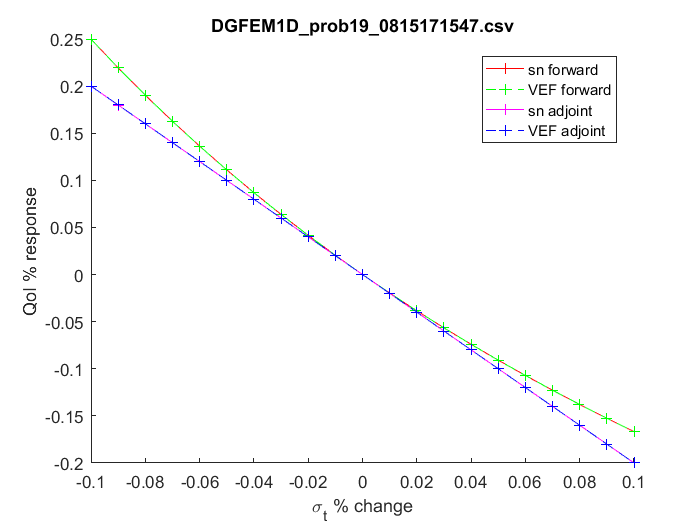
\includegraphics[width=.8\linewidth]{figures/19sigtSens.png}
  \caption{Uniform perturbation system with initial $\sigt=2$, $\sigs=1$. }
  \label{fig:sfig1}
\end{subfigure}%
\begin{subfigure}{.5\textwidth}
  \centering
  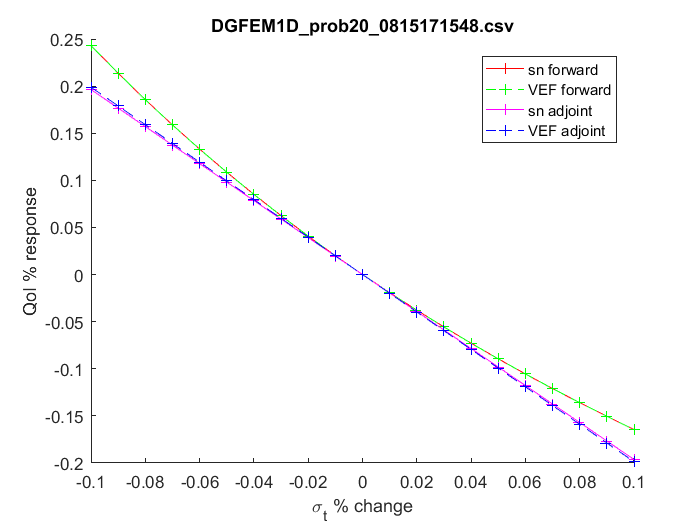
\includegraphics[width=.8\linewidth]{figures/20sigtSens.png}
  \caption{Uniform perturbation system with initial $\sigt=1$, $\sigs=0.5$. }
  \label{fig:sfig2}
\end{subfigure}
\begin{subfigure}{.5\textwidth}
  \centering
  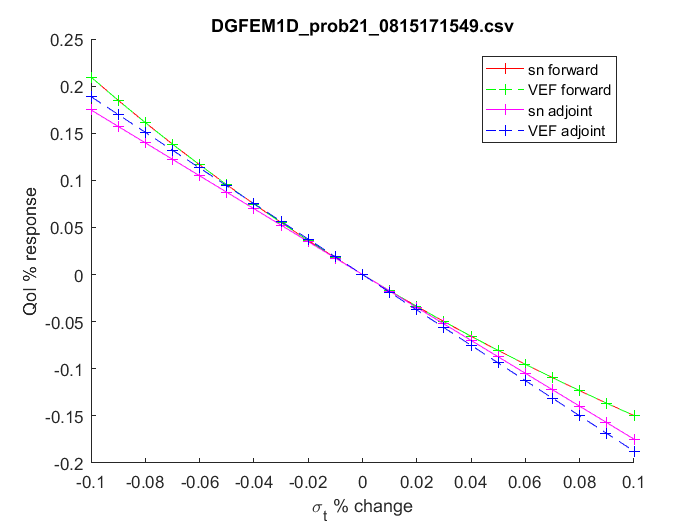
\includegraphics[width=.8\linewidth]{figures/21sigtSens.png}
  \caption{Uniform perturbation system with initial $\sigt=0.5$, $\sigs=0.25$.}
  \label{fig:sfig3}
\end{subfigure}
\caption{Plots of $\sigt$ perturbation sensitivity for uniformly perturbed system.}
\label{fig:fig}
\end{figure}

\begin{figure}[H]
\label{HomoPerts}
\centering
\begin{subfigure}{.5\textwidth}
  \centering
  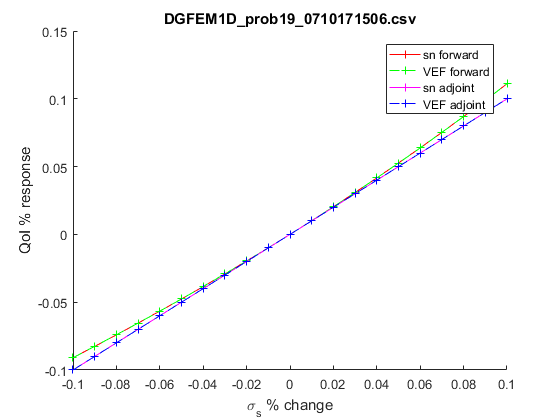
\includegraphics[width=.8\linewidth]{figures/19sigsSens.png}
  \caption{Uniform perturbation system with initial $\sigt=2$, $\sigs=1$.}
  \label{fig:sfig1}
\end{subfigure}%
\begin{subfigure}{.5\textwidth}
  \centering
  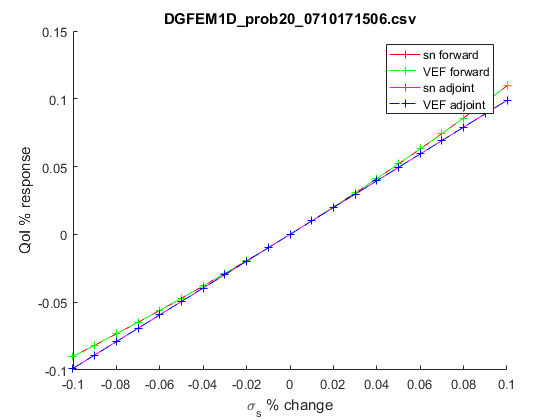
\includegraphics[width=.8\linewidth]{figures/20sigsSens.png}
  \caption{Uniform perturbation system with initial $\sigt=1$, $\sigs=0.5$.}
  \label{fig:sfig2}
\end{subfigure}
\begin{subfigure}{.5\textwidth}
  \centering
  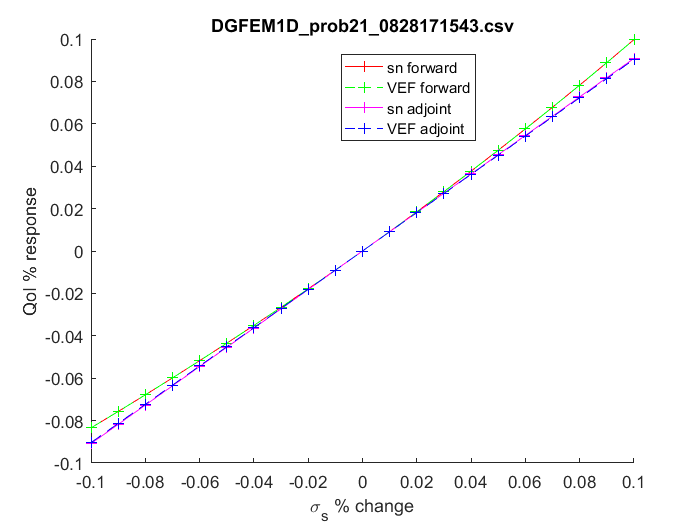
\includegraphics[width=.8\linewidth]{figures/21sigsSens.png}
  \caption{Uniform perturbation system with initial $\sigt=0.5$, $\sigs=0.25$.}
  \label{fig:sfig3}
\end{subfigure}
\caption{Plots of $\sigs$ perturbation sensitivity for uniformly perturbed system.}
\label{fig:fig}
\end{figure}

\begin{figure}[H]
\label{HomoPertq}
\centering
\begin{subfigure}{.5\textwidth}
  \centering
  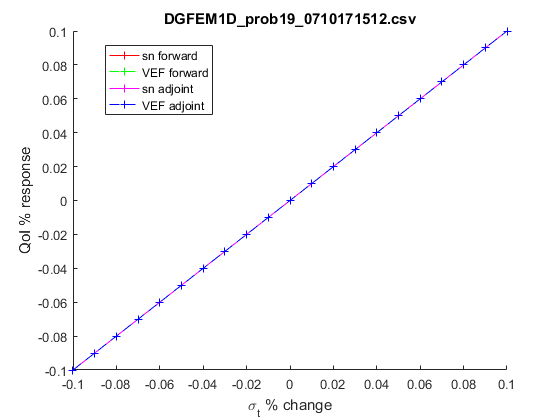
\includegraphics[width=.8\linewidth]{figures/19qSens.png}
  \caption{Uniform perturbation system with initial $\sigt=2$, $\sigs=1$}
  \label{fig:sfig1}
\end{subfigure}%
\begin{subfigure}{.5\textwidth}
  \centering
  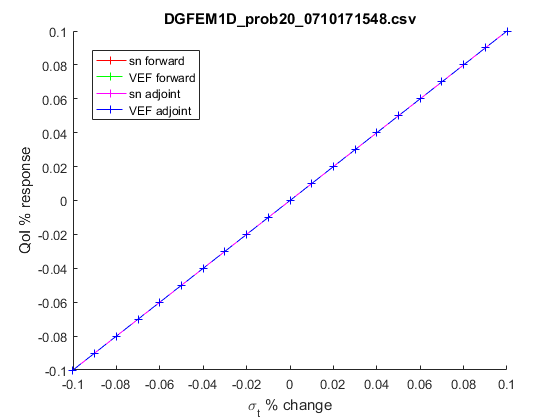
\includegraphics[width=.8\linewidth]{figures/20qSens.png}
  \caption{Uniform perturbation system with initial $\sigt=1$, $\sigs=0.5$}
  \label{fig:sfig2}
\end{subfigure}
\begin{subfigure}{.5\textwidth}
  \centering
  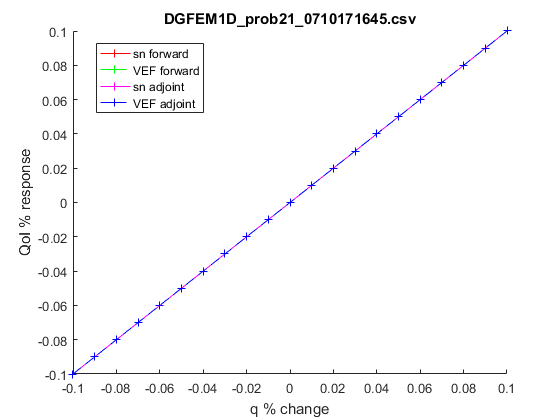
\includegraphics[width=.8\linewidth]{figures/21qSens.png}
  \caption{Uniform perturbation system with initial $\sigt=0.5$, $\sigs=0.25$}
  \label{fig:sfig3}
\end{subfigure}
\caption{Plots of source perturbation sensitivity for uniformly perturbed system.}
\label{fig:fig}
\end{figure}

%%%%%%%----------------------------------------------------------------------------------------------
\subsection{Homogeneous initial system, Non-Uniform Perturbations}
%%%%%%%----------------------------------------------------------------------------------------------

The next test case has the same initial conditions as the previous homogeneous case. however the system is perturbed into a inhomogeneous system. The system is split into 5 equal widths. The first, third, and fifth sections (corresponding to the center and the end sections) have the relevant variable perturbed in one direction, while the other two segments are perturbed in the opposite direction. The result is a system that is inhomogeneous, but with regular variations and symmetric about the midpoint. The \qoi is also retained from the previous case.

\begin{figure}[H]
\label{InHomoPertt}
\centering
\begin{subfigure}{.5\textwidth}
  \centering
  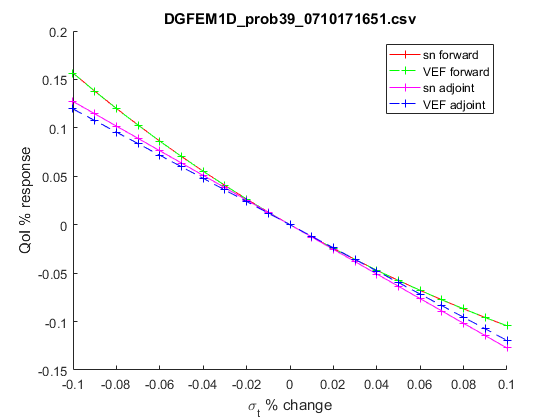
\includegraphics[width=.8\linewidth]{figures/39sigtSens.png}
  \caption{Inhomogeneous perturbation system with initial $\sigt=2$, $\sigs=1$}
  \label{fig:sfig1}
\end{subfigure}%
\begin{subfigure}{.5\textwidth}
  \centering
  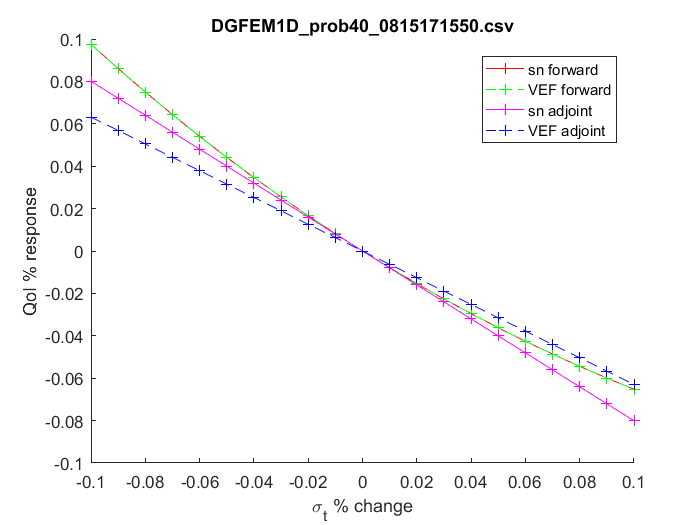
\includegraphics[width=.8\linewidth]{figures/40sigtSens.png}
  \caption{Inhomogeneous perturbation system with initial $\sigt=1$, $\sigs=0.5$}
  \label{fig:sfig2}
\end{subfigure}
\begin{subfigure}{.5\textwidth}
  \centering
  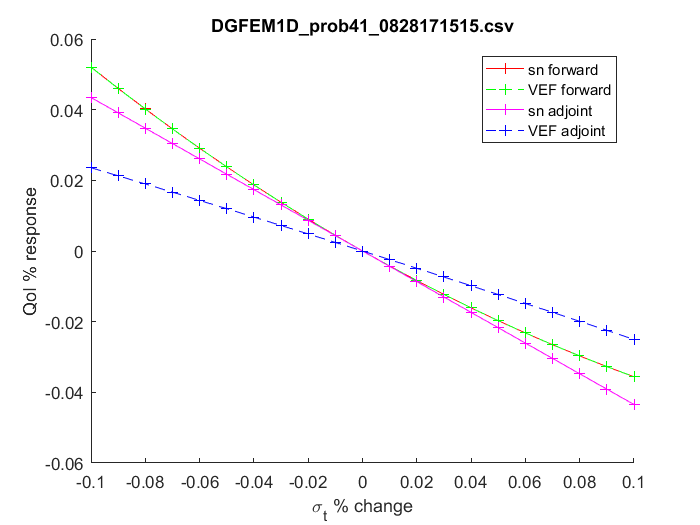
\includegraphics[width=.8\linewidth]{figures/41sigtSens.png}
  \caption{Inhomogeneous perturbation system with initial $\sigt=0.5$, $\sigs=0.25$}
  \label{fig:sfig3}
\end{subfigure}
\caption{Plots of $\sigt$ perturbation sensitivity for non-uniformly perturbed system.}
\label{fig:fig}
\end{figure}

\begin{figure}[H]
\label{InHomoPerts}
\centering
\begin{subfigure}{.5\textwidth}
  \centering
  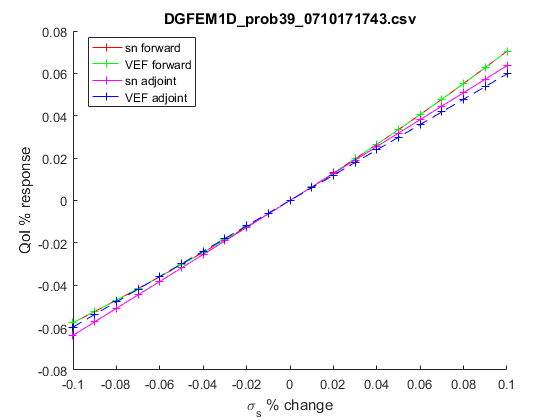
\includegraphics[width=.8\linewidth]{figures/39sigsSens.png}
  \caption{Inhomogeneous perturbation system with initial $\sigt=2$, $\sigs=1$}
  \label{fig:sfig1}
\end{subfigure}%
\begin{subfigure}{.5\textwidth}
  \centering
  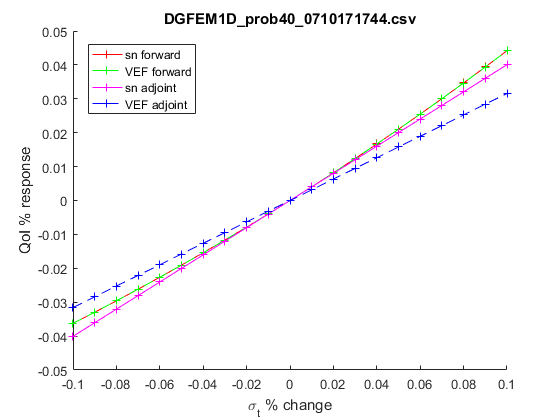
\includegraphics[width=.8\linewidth]{figures/40sigsSens.png}
  \caption{Inhomogeneous perturbation system with initial $\sigt=1$, $\sigs=0.5$}
  \label{fig:sfig2}
\end{subfigure}
\begin{subfigure}{.5\textwidth}
  \centering
  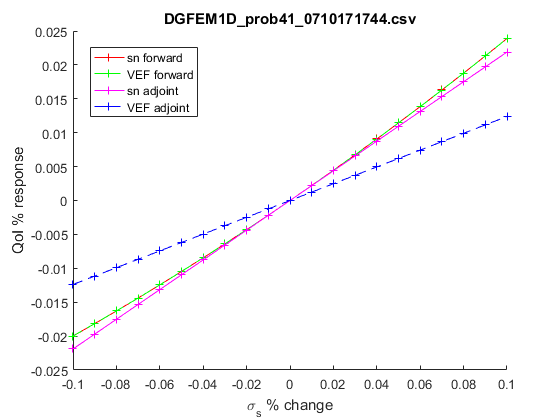
\includegraphics[width=.8\linewidth]{figures/41sigsSens.png}
  \caption{Inhomogeneous perturbation system with initial $\sigt=0.5$, $\sigs=0.25$}
  \label{fig:sfig3}
\end{subfigure}
\caption{Plots of $\sigs$ perturbation sensitivity for non-uniformly perturbed system.}
\label{fig:fig}
\end{figure}

\begin{figure}[H]
\label{InHomoPertq}
\centering
\begin{subfigure}{.5\textwidth}
  \centering
  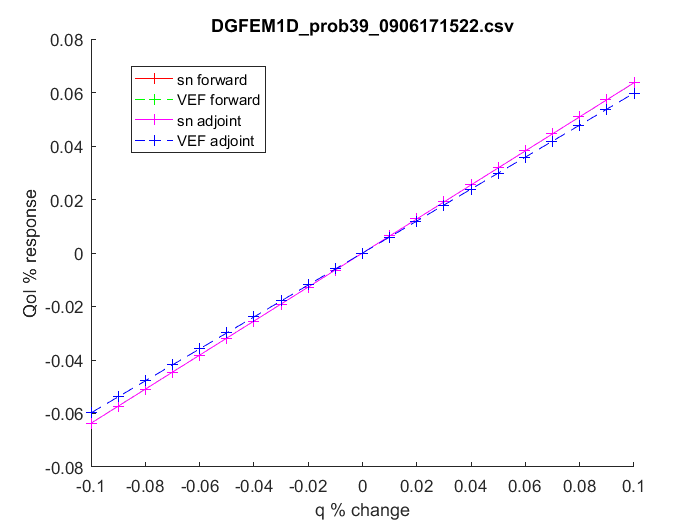
\includegraphics[width=.8\linewidth]{figures/39qSens.png}
  \caption{Inhomogeneous perturbation system with initial $\sigt=2$, $\sigs=1$}
  \label{fig:sfig1}
\end{subfigure}%
\begin{subfigure}{.5\textwidth}
  \centering
  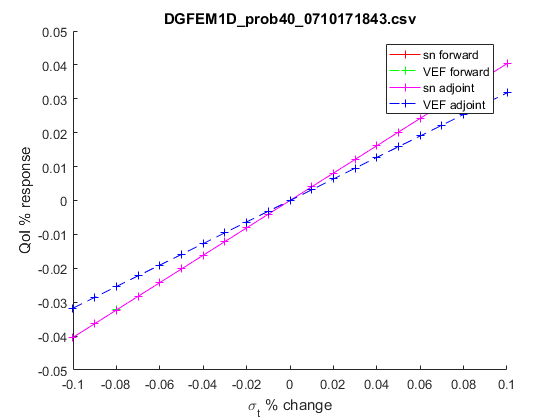
\includegraphics[width=.8\linewidth]{figures/40qSens.png}
  \caption{Inhomogeneous perturbation system with initial $\sigt=1$, $\sigs=0.5$}
  \label{fig:sfig2}
\end{subfigure}
\begin{subfigure}{.5\textwidth}
  \centering
  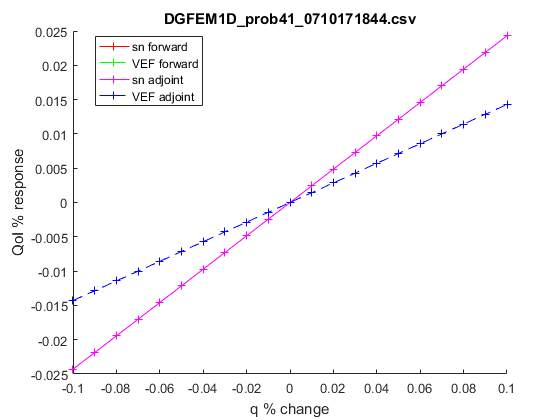
\includegraphics[width=.8\linewidth]{figures/41qSens.png}
  \caption{Inhomogeneous perturbation system with initial $\sigt=0.5$, $\sigs=0.25$}
  \label{fig:sfig3}
\end{subfigure}
\caption{Plots of source perturbation sensitivity for non-uniformly perturbed system.}
\label{fig:fig}
\end{figure}

%%%%%%%----------------------------------------------------------------------------------------------
\subsection{Streaming system}
%%%%%%%----------------------------------------------------------------------------------------------
To generate a streaming system, we retain the 5 equal width sectioning of the previous inhomogeneous example, but the second and fourth sections are converted to streaming regions ($\sigt \approx 0 $). Leaving three neutron producing sections separated by two streaming gaps. The \qoi remains as the total neutron count in the center fifth section.

\begin{figure}[H]
\label{InHomoPertt}
\centering
\begin{subfigure}{.5\textwidth}
  \centering
  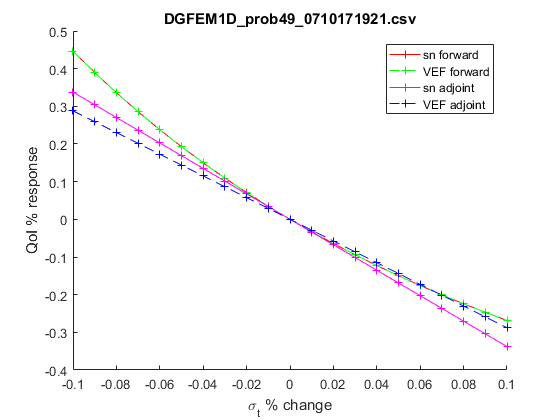
\includegraphics[width=.8\linewidth]{figures/49sigtSens.png}
  \caption{Streaming perturbation system with initial $\sigt=2$, $\sigs=1$}
  \label{fig:sfig1}
\end{subfigure}%
\begin{subfigure}{.5\textwidth}
  \centering
  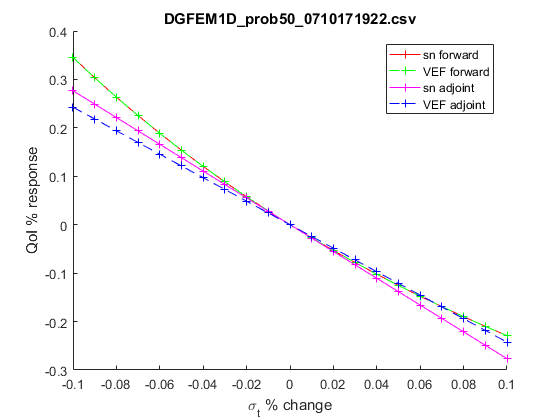
\includegraphics[width=.8\linewidth]{figures/50sigtSens.png}
  \caption{Streaming perturbation system with initial $\sigt=1$, $\sigs=0.5$}
  \label{fig:sfig2}
\end{subfigure}
\begin{subfigure}{.5\textwidth}
  \centering
  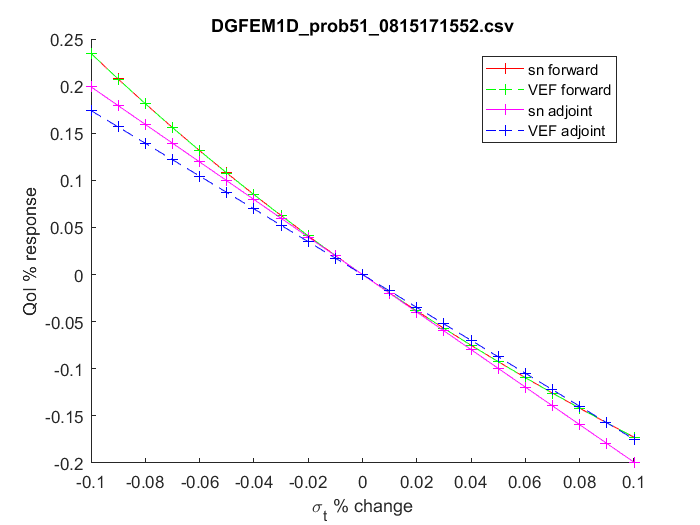
\includegraphics[width=.8\linewidth]{figures/51sigtSens.png}
  \caption{Streaming perturbation system with initial $\sigt=0.5$, $\sigs=0.25$}
  \label{fig:sfig3}
\end{subfigure}
\caption{Plots of $\sigt$ perturbation sensitivity for perturbed streaming system.}
\label{fig:fig}
\end{figure}

\begin{figure}[H]
\label{InHomoPerts}
\centering
\begin{subfigure}{.5\textwidth}
  \centering
  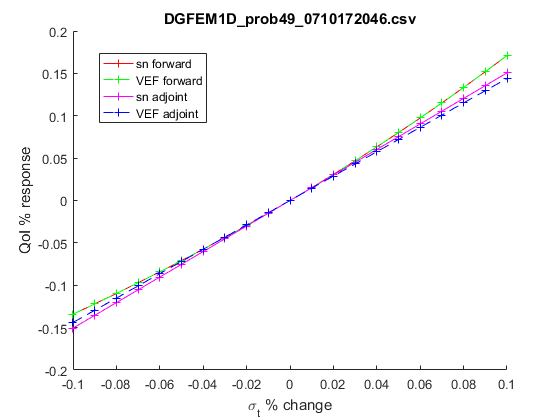
\includegraphics[width=.8\linewidth]{figures/49sigsSens.png}
  \caption{Streaming perturbation system with initial $\sigt=2$, $\sigs=1$}
  \label{fig:sfig1}
\end{subfigure}%
\begin{subfigure}{.5\textwidth}
  \centering
  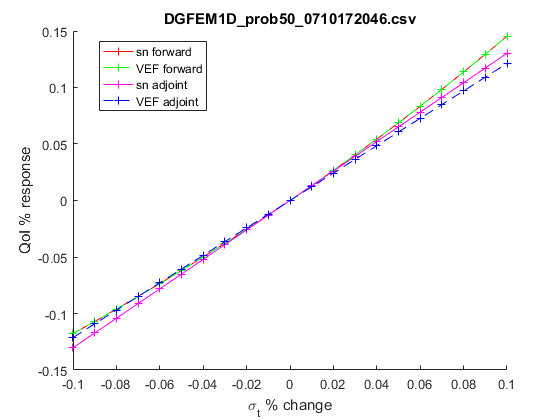
\includegraphics[width=.8\linewidth]{figures/50sigsSens.png}
  \caption{Streaming perturbation system with initial $\sigt=1$, $\sigs=0.5$}
  \label{fig:sfig2}
\end{subfigure}
\begin{subfigure}{.5\textwidth}
  \centering
  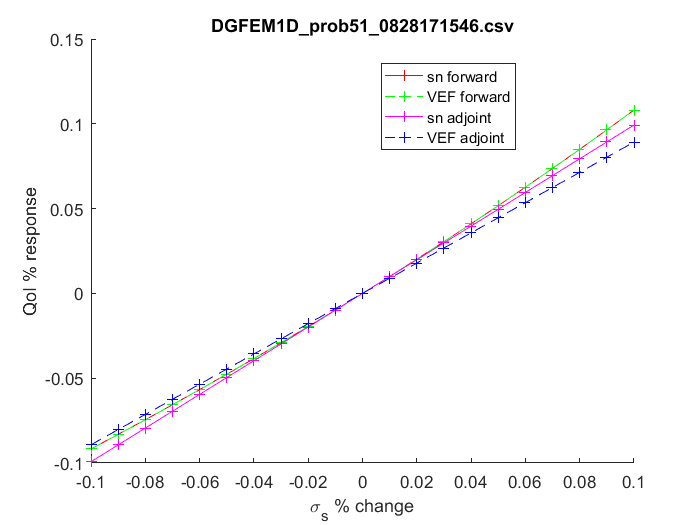
\includegraphics[width=.8\linewidth]{figures/51sigsSens.png}
  \caption{Streaming perturbation system with initial $\sigt=0.5$, $\sigs=0.25$}
  \label{fig:sfig3}
\end{subfigure}
\caption{Plots of $\sigs$ perturbation sensitivity for perturbed streaming system.}
\label{fig:fig}
\end{figure}

\begin{figure}[H]
\label{InHomoPertq}
\centering
\begin{subfigure}{.5\textwidth}
  \centering
  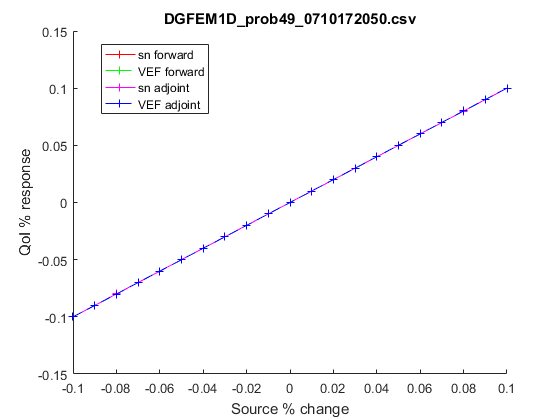
\includegraphics[width=.8\linewidth]{figures/49qSens.png}
  \caption{Streaming perturbation system with initial $\sigt=2$, $\sigs=1$}
  \label{fig:sfig1}
\end{subfigure}%
\begin{subfigure}{.5\textwidth}
  \centering
  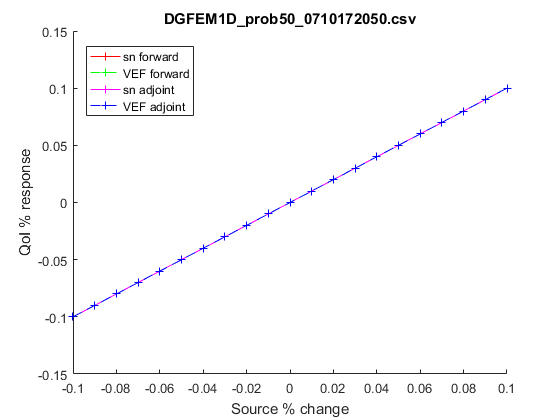
\includegraphics[width=.8\linewidth]{figures/50qSens.png}
  \caption{Streaming perturbation system with initial $\sigt=1$, $\sigs=0.5$}
  \label{fig:sfig2}
\end{subfigure}
\begin{subfigure}{.5\textwidth}
  \centering
  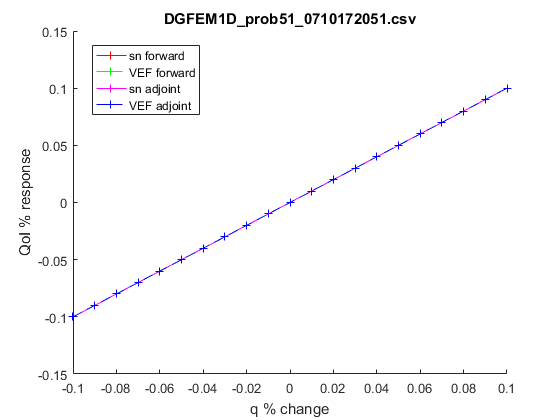
\includegraphics[width=.8\linewidth]{figures/51qSens.png}
  \caption{Streaming perturbation system with initial $\sigt=0.5$, $\sigs=0.25$}
  \label{fig:sfig3}
\end{subfigure}
\caption{Plots of source perturbation sensitivity for perturbed streaming system.}
\label{fig:fig}
\end{figure}

\jcr{generally speaking, your figure captions should be more descriptive than they currently are. And it should be clear to which test case they below to}

%%%%%%%%%%%%%%%%%%%%%%%%%%%%%%%%%%%%%%%%%%%%%%%%%%%%%%%%%%%%%%%%%%%%%%%%%%%%%%%%%%%%%%%%%%%%%%%%%%%%%
\section{Goals of the Research}
%%%%%%%%%%%%%%%%%%%%%%%%%%%%%%%%%%%%%%%%%%%%%%%%%%%%%%%%%%%%%%%%%%%%%%%%%%%%%%%%%%%%%%%%%%%%%%%%%%%%%

\begin{itemize}
\item Formulate an adjoint equation based on the VET transport formulation, including derivation of appropriate BC for the adjoint unknown.
\item Define the inner products required for first-order sensitivity calculations using the VET formulation for perturbations in cross sections, sources, and incident flux, assuming an unperturbed Eddington Tensor
\item Derive terms that were lost in the first-order adjoint sensitivity formulation due to the assumption that the Eddington remains unperturbed. 
\item Implement the Sn and VET adjoint methods in a 1D FEM solver. 
\item Using 1D test cases, compare the sensitivity values yielded by the VET adjoint method to those obtained by the standard Sn adjoint, as well as sensitivity obtained directly by multiple forward system solves in both Sn and VET.
%\item Consider the alternate boundary conditions presented in Wieselquest. If promise is shown, derive the sensitivity inner products using this boundary condition. Repeat select test cases of the 1D implementation.
\end{itemize}

\newpage

%%%%%%%----------------------------------------------------------------------------------------------
%%%%%%%----------------------------------------------------------------------------------------------
%%%%%%%----------------------------------------------------------------------------------------------
%%%%%%%----------------------------------------------------------------------------------------------
%%%%%%%----------------------------------------------------------------------------------------------
%%%%%%%----------------------------------------------------------------------------------------------
%%%%%%%----------------------------------------------------------------------------------------------
%%%%%%%----------------------------------------------------------------------------------------------
%%%%%%%----------------------------------------------------------------------------------------------

\newpage

%%%%%%
%%%%%%%----------------------------------------------------------------------------------------------

\bibliography{IanProp} 
\bibliographystyle{ieeetr}

%%%%%%%----------------------------------------------------------------------------------------------
\end{document}